\documentclass{standalone}
%
\usepackage{tikz}
\usepackage{xcolor}
%
\definecolor{craterm}{HTML}{616060}
%
\title{Squares}
\begin{document}
	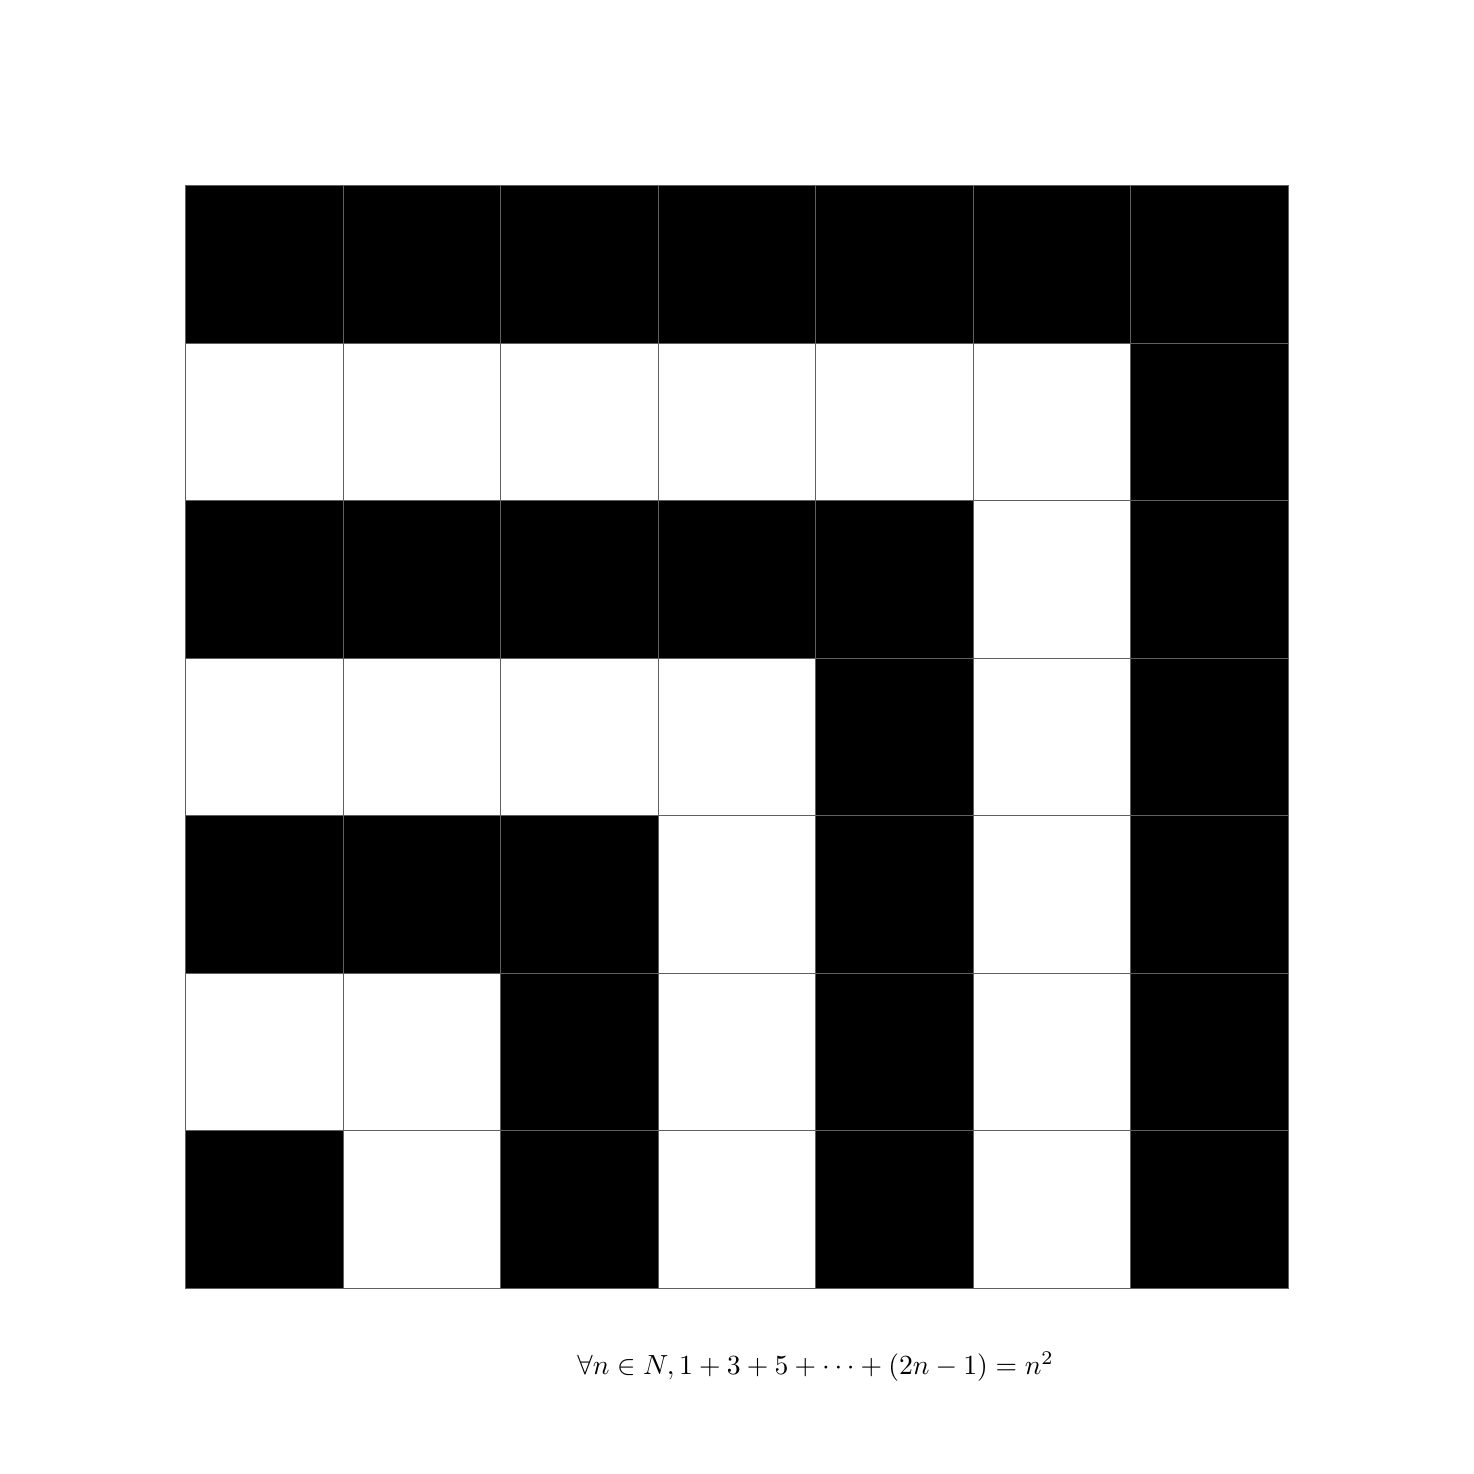
\begin{tikzpicture}
		\begin{scope}[scale=2]
			\draw [color=white,fill=white] (-1,-1) rectangle (8,8);
			\foreach \x in {0,2,4,6}
				\draw [fill=black] (\x,0) rectangle (\x+1,1);
			\foreach \x in {2,4,6}
				\draw [fill=black] (\x,1) rectangle (\x+1,2);
			\foreach \x in {0,1,2,4,6}
				\draw [fill=black] (\x,2) rectangle (\x+1,3);
			\foreach \x in {4,6}
				\draw [fill=black] (\x,3) rectangle (\x+1,4);
			\foreach \x in {0,1,2,3,4,6}
				\draw [fill=black] (\x,4) rectangle (\x+1,5);
			\draw [fill=black] (6,5) rectangle (7,6);
			\foreach \x in {0,1,...,6}
				\draw [fill=black] (\x,6) rectangle (\x+1,7);
			\foreach \x in {0,1,...,6}
				\foreach \y in {0,1,...,6}
					\draw [color=craterm] (\x,\y) rectangle (\x+1,\y+1);
		\end{scope}
		%
		\begin{scope}[shift={(0,-1)}]
			\node at (8,0) {$\forall n \in N, 1+3+5+\cdots+(2n-1) = n^2$};
		\end{scope}
	\end{tikzpicture}
\end{document}